\section{Results}

\subsection{Main Results}

Table~\ref{tab:main} reports F1, B1, and J across four question categories on the LoCoMo test set.

\begin{table}[t]
\centering
\caption{Main results on LoCoMo (20/80 train/test split, 1{,}232 test QA pairs, adversarial category excluded). F1: token-level F1; B1: BLEU-1; J: LLM-as-judge accuracy (GPT-4o mini). Best non-oracle results per column in \textbf{bold}. Oracle results in \textit{italics}.}
\label{tab:main}
\small
\setlength{\tabcolsep}{2.8pt}
\begin{tabular}{l @{\hskip 5pt} ccc @{\hskip 3pt} ccc @{\hskip 3pt} ccc @{\hskip 3pt} ccc @{\hskip 3pt} ccc}
\toprule
 & \multicolumn{3}{c}{\cellcolor{hdrOverall}\textbf{Overall}} & \multicolumn{3}{c}{\cellcolor{hdrMH}\textbf{Multi-hop}} & \multicolumn{3}{c}{\cellcolor{hdrSH}\textbf{Single-hop}} & \multicolumn{3}{c}{\cellcolor{hdrTemp}\textbf{Temporal}} & \multicolumn{3}{c}{\cellcolor{hdrOD}\textbf{Open-domain}} \\
\textbf{Method} & \cellcolor{hdrOverall}F1 & \cellcolor{hdrOverall}B1 & \cellcolor{hdrOverall}J & \cellcolor{hdrMH}F1 & \cellcolor{hdrMH}B1 & \cellcolor{hdrMH}J & \cellcolor{hdrSH}F1 & \cellcolor{hdrSH}B1 & \cellcolor{hdrSH}J & \cellcolor{hdrTemp}F1 & \cellcolor{hdrTemp}B1 & \cellcolor{hdrTemp}J & \cellcolor{hdrOD}F1 & \cellcolor{hdrOD}B1 & \cellcolor{hdrOD}J \\
\midrule
\multicolumn{16}{l}{\textit{Context-based} \hfill \scriptsize No retrieval; answers from raw context or gold evidence} \\[2pt]
Full Context & 24.2 & 19.7 & 45.7 & 19.7 & 15.8 & 40.4 & 23.9 & 19.0 & 45.7 & 16.2 & 12.5 & 37.3 & 27.0 & 22.3 & 48.6 \\
\rowcolor{rowOracle}Oracle$^\dagger$ & \textit{31.3} & \textit{25.7} & \textit{60.8} & \textit{34.3} & \textit{27.9} & \textit{63.1} & \textit{31.6} & \textit{25.9} & \textit{62.2} & \textit{35.4} & \textit{29.7} & \textit{65.2} & \textit{29.5} & \textit{24.3} & \textit{59.0} \\
\midrule
\multicolumn{16}{l}{\textit{Retrieval-based} \hfill \scriptsize Heuristic or similarity-based retrieval; no RL training} \\[2pt]
RAG (BM25) & 29.9 & 25.3 & 49.8 & 19.0 & 14.6 & 28.1 & 22.6 & 17.6 & 30.6 & 11.2 & 8.8 & 25.1 & \textbf{38.7} & \textbf{33.9} & \textbf{67.3} \\
RAG (Embedding) & 29.5 & 24.3 & 49.6 & 21.1 & 15.8 & 31.5 & 21.8 & 17.3 & 32.4 & 12.1 & 8.8 & 24.2 & 37.2 & 31.7 & 65.1 \\
Semantic XPath & 18.5 & 14.4 & 39.8 & 25.9 & 20.4 & 53.7 & 21.3 & 16.5 & 45.1 & 29.8 & 24.9 & 49.0 & 13.4 & 10.2 & 31.6 \\
\midrule
\multicolumn{16}{l}{\textit{RL-based} \hfill \scriptsize Policy trained with GRPO from downstream QA reward} \\[2pt]
Memory R1 & 27.4 & 22.7 & 53.9 & 22.5 & 17.4 & 50.1 & \textbf{27.7} & \textbf{23.6} & \textbf{54.9} & 20.8 & 16.5 & 48.0 & 30.0 & 25.2 & 55.7 \\
\rowcolor{rowOurs}\textsc{Struct Memory-R1} (Ours)$^*$ & \textbf{30.4} & \textbf{25.4} & \textbf{54.4} & \textbf{31.5} & \textbf{26.8} & \textbf{56.2} & 27.1 & 21.7 & 53.7 & \textbf{34.6} & \textbf{28.6} & \textbf{58.6} & 30.6 & 25.8 & 53.4 \\
\bottomrule
\end{tabular}
\vspace{2pt}

{\footnotesize $^\dagger$Uses gold evidence annotations from LoCoMo (upper bound). $^*$Uses oracle human-judged structured data; results may overestimate performance achievable with automatically induced structure.}
\end{table}

\textsc{Struct Memory-R1} achieves the highest overall F1 (30.4), B1 (25.4), and J (54.4) among non-oracle methods. The gains are concentrated in multi-hop and temporal reasoning, where tree-structured retrieval enables the model to navigate related facts through shared ancestors rather than scoring each memory independently. On multi-hop questions, our method improves F1 by 9.0 points over Memory~R1 (31.5 vs.\ 22.5) and J by 6.1 points (56.2 vs.\ 50.1). On temporal questions, the improvement is even larger: 13.8 F1 points and 10.6 J points over Memory~R1. These categories require combining information across sessions or reasoning about time, both of which benefit from the hierarchical grouping that tree structure provides.

The picture is different for single-hop and open-domain questions. Memory~R1 edges out our method on single-hop (27.7 vs.\ 27.1 F1, 23.6 vs.\ 21.7 B1, 54.9 vs.\ 53.7 J), where flat retrieval is sufficient because the answer resides in a single memory entry and tree navigation adds no benefit. On open-domain questions, RAG~(BM25) achieves the highest F1 (38.7), B1 (33.9), and J (67.3) by a wide margin. Open-domain questions often require broad factual recall that favors high-coverage keyword matching over focused structural navigation. Our method nonetheless outperforms Memory~R1 on open-domain F1 (30.6 vs.\ 30.0), suggesting that tree-organized memory retains some advantage even for general questions.

An interesting pattern appears in the retrieval-based baselines. Semantic XPath achieves substantially higher J than both RAG methods on single-hop (45.1 vs.\ 30.6/32.4) and multi-hop (53.7 vs.\ 28.1/31.5) despite comparable or lower F1 and B1. This indicates that structured retrieval surfaces contextually richer evidence that helps the model produce semantically correct answers even when lexical overlap with the gold answer is limited. The same F1--J divergence appears in our method relative to RAG: our J scores are consistently higher than RAG across multi-hop, single-hop, and temporal categories, even when lexical metrics are comparable.

We note that our current results use oracle human-judged structured data for memory construction rather than automatically induced structure. This means the Memory Manager component has not yet been trained end-to-end, and the reported numbers may overestimate the performance achievable with fully automatic structure induction. The ablation study below examines the contribution of each component under this setting.

\subsection{Ablation Study}

\begin{figure}[t]
\centering
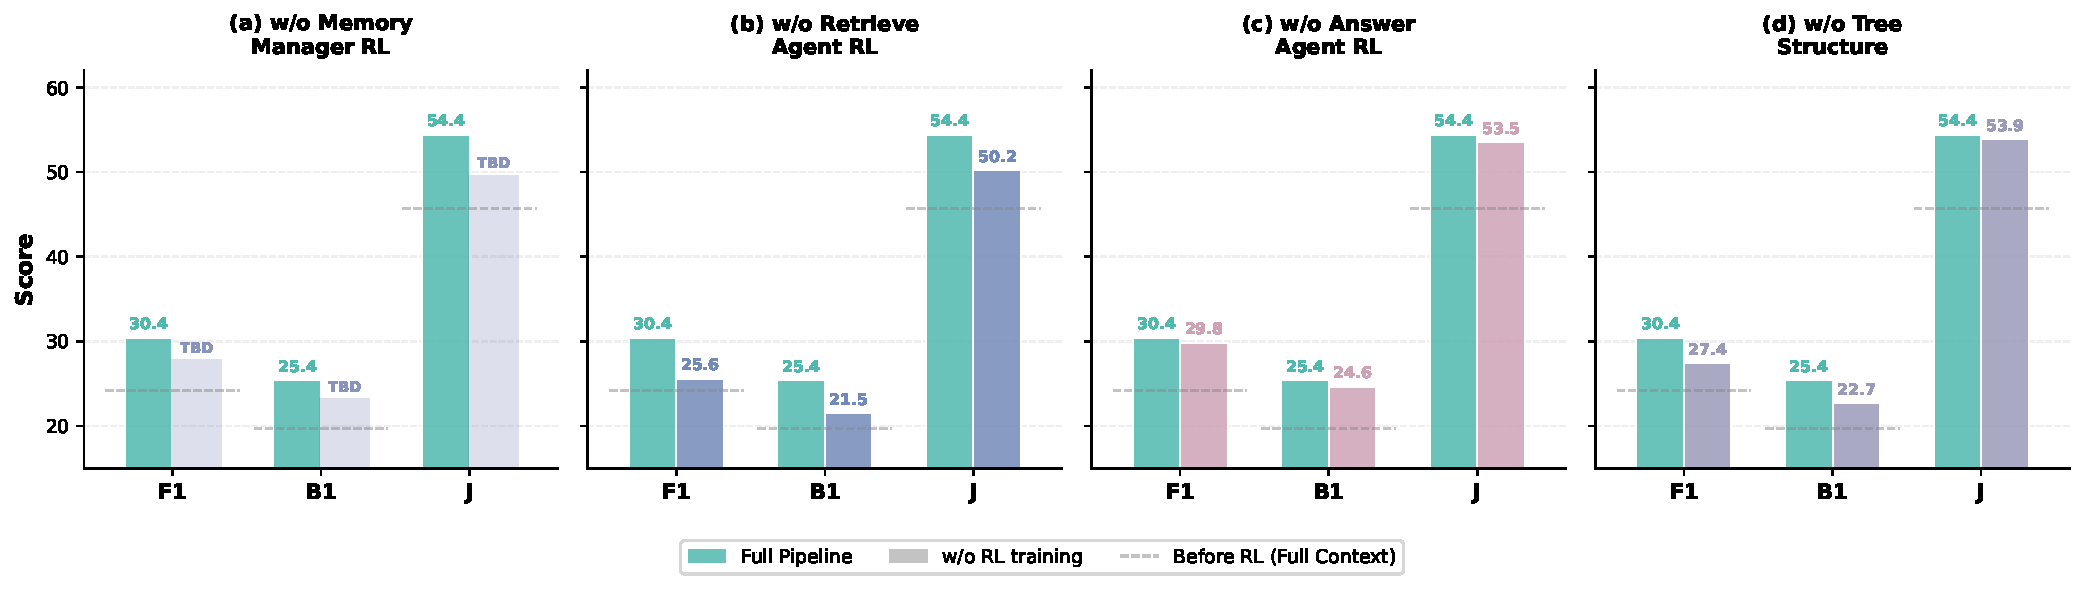
\includegraphics[width=\textwidth]{figures/ablation_figure.pdf}
\caption{Ablation analysis of \textsc{Struct Memory-R1}. Each subfigure shows the effect of disabling RL training for one component: (a) Memory Manager, (b) Retrieve Agent, (c) Answer Agent, and (d) replacing tree structure with flat memory. Teal bars show the full pipeline; colored bars show the ablated variant. Grey dashed lines indicate the before-RL baseline (Full Context). Note that ``w/o'' disables RL fine-tuning for the component, not the component itself. The Memory Manager ablation (hatched bars) is pending completion.}
\label{fig:ablation}
\end{figure}

Figure~\ref{fig:ablation} shows the effect of disabling RL training for each component. Disabling Retrieve Agent RL (Figure~\ref{fig:ablation}b) causes the largest degradation, dropping F1 from 30.4 to 25.6, B1 from 25.4 to 21.5, and J from 54.4 to 50.2. This confirms that learned tree navigation is the most critical component: without it, the system falls back to heuristic retrieval over tree leaves and loses the ability to plan structured search paths.

Disabling Answer Agent RL (Figure~\ref{fig:ablation}c) produces only a modest drop (F1 to 29.8, B1 to 24.6, J to 53.5), suggesting that the base Qwen2.5-3B-Instruct model is already a reasonably capable reader when provided with well-retrieved evidence. The primary bottleneck in our pipeline is retrieval quality, not answer generation.

Replacing tree structure with flat memory (Figure~\ref{fig:ablation}d) while keeping all RL components yields numbers that closely match Memory~R1 (F1 27.4, B1 22.7, J 53.9), as expected since this ablation is architecturally equivalent to Memory~R1. The 3.0-point F1 gap between flat and tree-structured retrieval demonstrates the value of hierarchical memory organization as an inductive bias for the retriever.

The Memory Manager RL ablation (Figure~\ref{fig:ablation}a) is ongoing and will quantify the contribution of RL-trained memory writing.
